\chapter{Interfacing a Potentiometer}
\thispagestyle{empty}
\label{potmeter}

\newcommand{\LocPotfig}{\Origin/user-code/pot/figures}
\newcommand{\LocPotscicode}{\Origin/user-code/pot/scilab}
\newcommand{\LocPotscibrief}[1]{{\tt
    \seqsplit{Origin/user-code/pot/scilab/#1}}, 
see \fnrefp{fn:file-loc}}
\newcommand{\LocPotardcode}{\Origin/user-code/pot/arduino}
\newcommand{\LocPotardbrief}[1]{{\tt
    \seqsplit{Origin/user-code/pot/arduino/#1}},
see \fnrefp{fn:file-loc}}

%%%%%%%%%%%%%%%python starts
\newcommand{\LocPotpycode}{\Origin/user-code/pot/python}
\newcommand{\LocPotpybrief}[1]{{\tt
    \seqsplit{Origin/user-code/pot/python/#1}},
see \fnrefp{fn:file-loc}}
%%%%%%%%%%%%%%%python ends

%%%%%%%%%%%%%%%julia starts
\newcommand{\LocPotjuliacode}{\Origin/user-code/pot/julia}
\newcommand{\LocPotjuliabrief}[1]{{\tt
    \seqsplit{Origin/user-code/pot/julia/#1}},
see \fnrefp{fn:file-loc}}
%%%%%%%%%%%%%%%julia ends

%%%%%%OpenModelica starts
\newcommand{\LocPotOpenModelicacode}{\Origin/user-code/pot/OpenModelica}
\newcommand{\LocPotOpenModelicabrief}[1]{{\tt
    \seqsplit{Origin/user-code/pot/OpenModelica/#1}},
see \fnrefp{fn:file-loc}}
%%%%%%OpenModelica ends

A potentiometer is a three-terminal variable resistor with two
terminals connected to the two ends of a resistor and one connected to
a sliding or rotating contact, termed as a wiper. The wiper can be
moved to vary the resistance, and hence the potential, between the
wiper and each terminal of the resistor. Thus, a potentiometer
functions as a variable potential divider. It finds wide application
in volume control, calibration and tuning circuits, motion control,
joysticks, etc.

In this chapter, we will perform an experiment to read the analog
values from a potentiometer mounted on the shield of \arduino\
board. The analog values read from the potentiometer will then be
used to control the actuation of other components.

\section{Preliminaries}
The shield provided with the kit has a 1K potentiometer mounted on
it. The mechanical contact at the middle terminal is rotated to vary
the resistance across the middle terminal and the two ends of the
potentiometer. With the fixed voltage across the two terminals of the
potentiometer, the position of the wiper determines the potential
across the middle terminal and either of the two end
terminals. Nowadays, digital potentiometer integrated circuits, which
vary resistance across two pins on the basis of the set value, are
also available.

\begin{figure}
\centering
\subfloat[Pictorial representation of a potentiometer]{
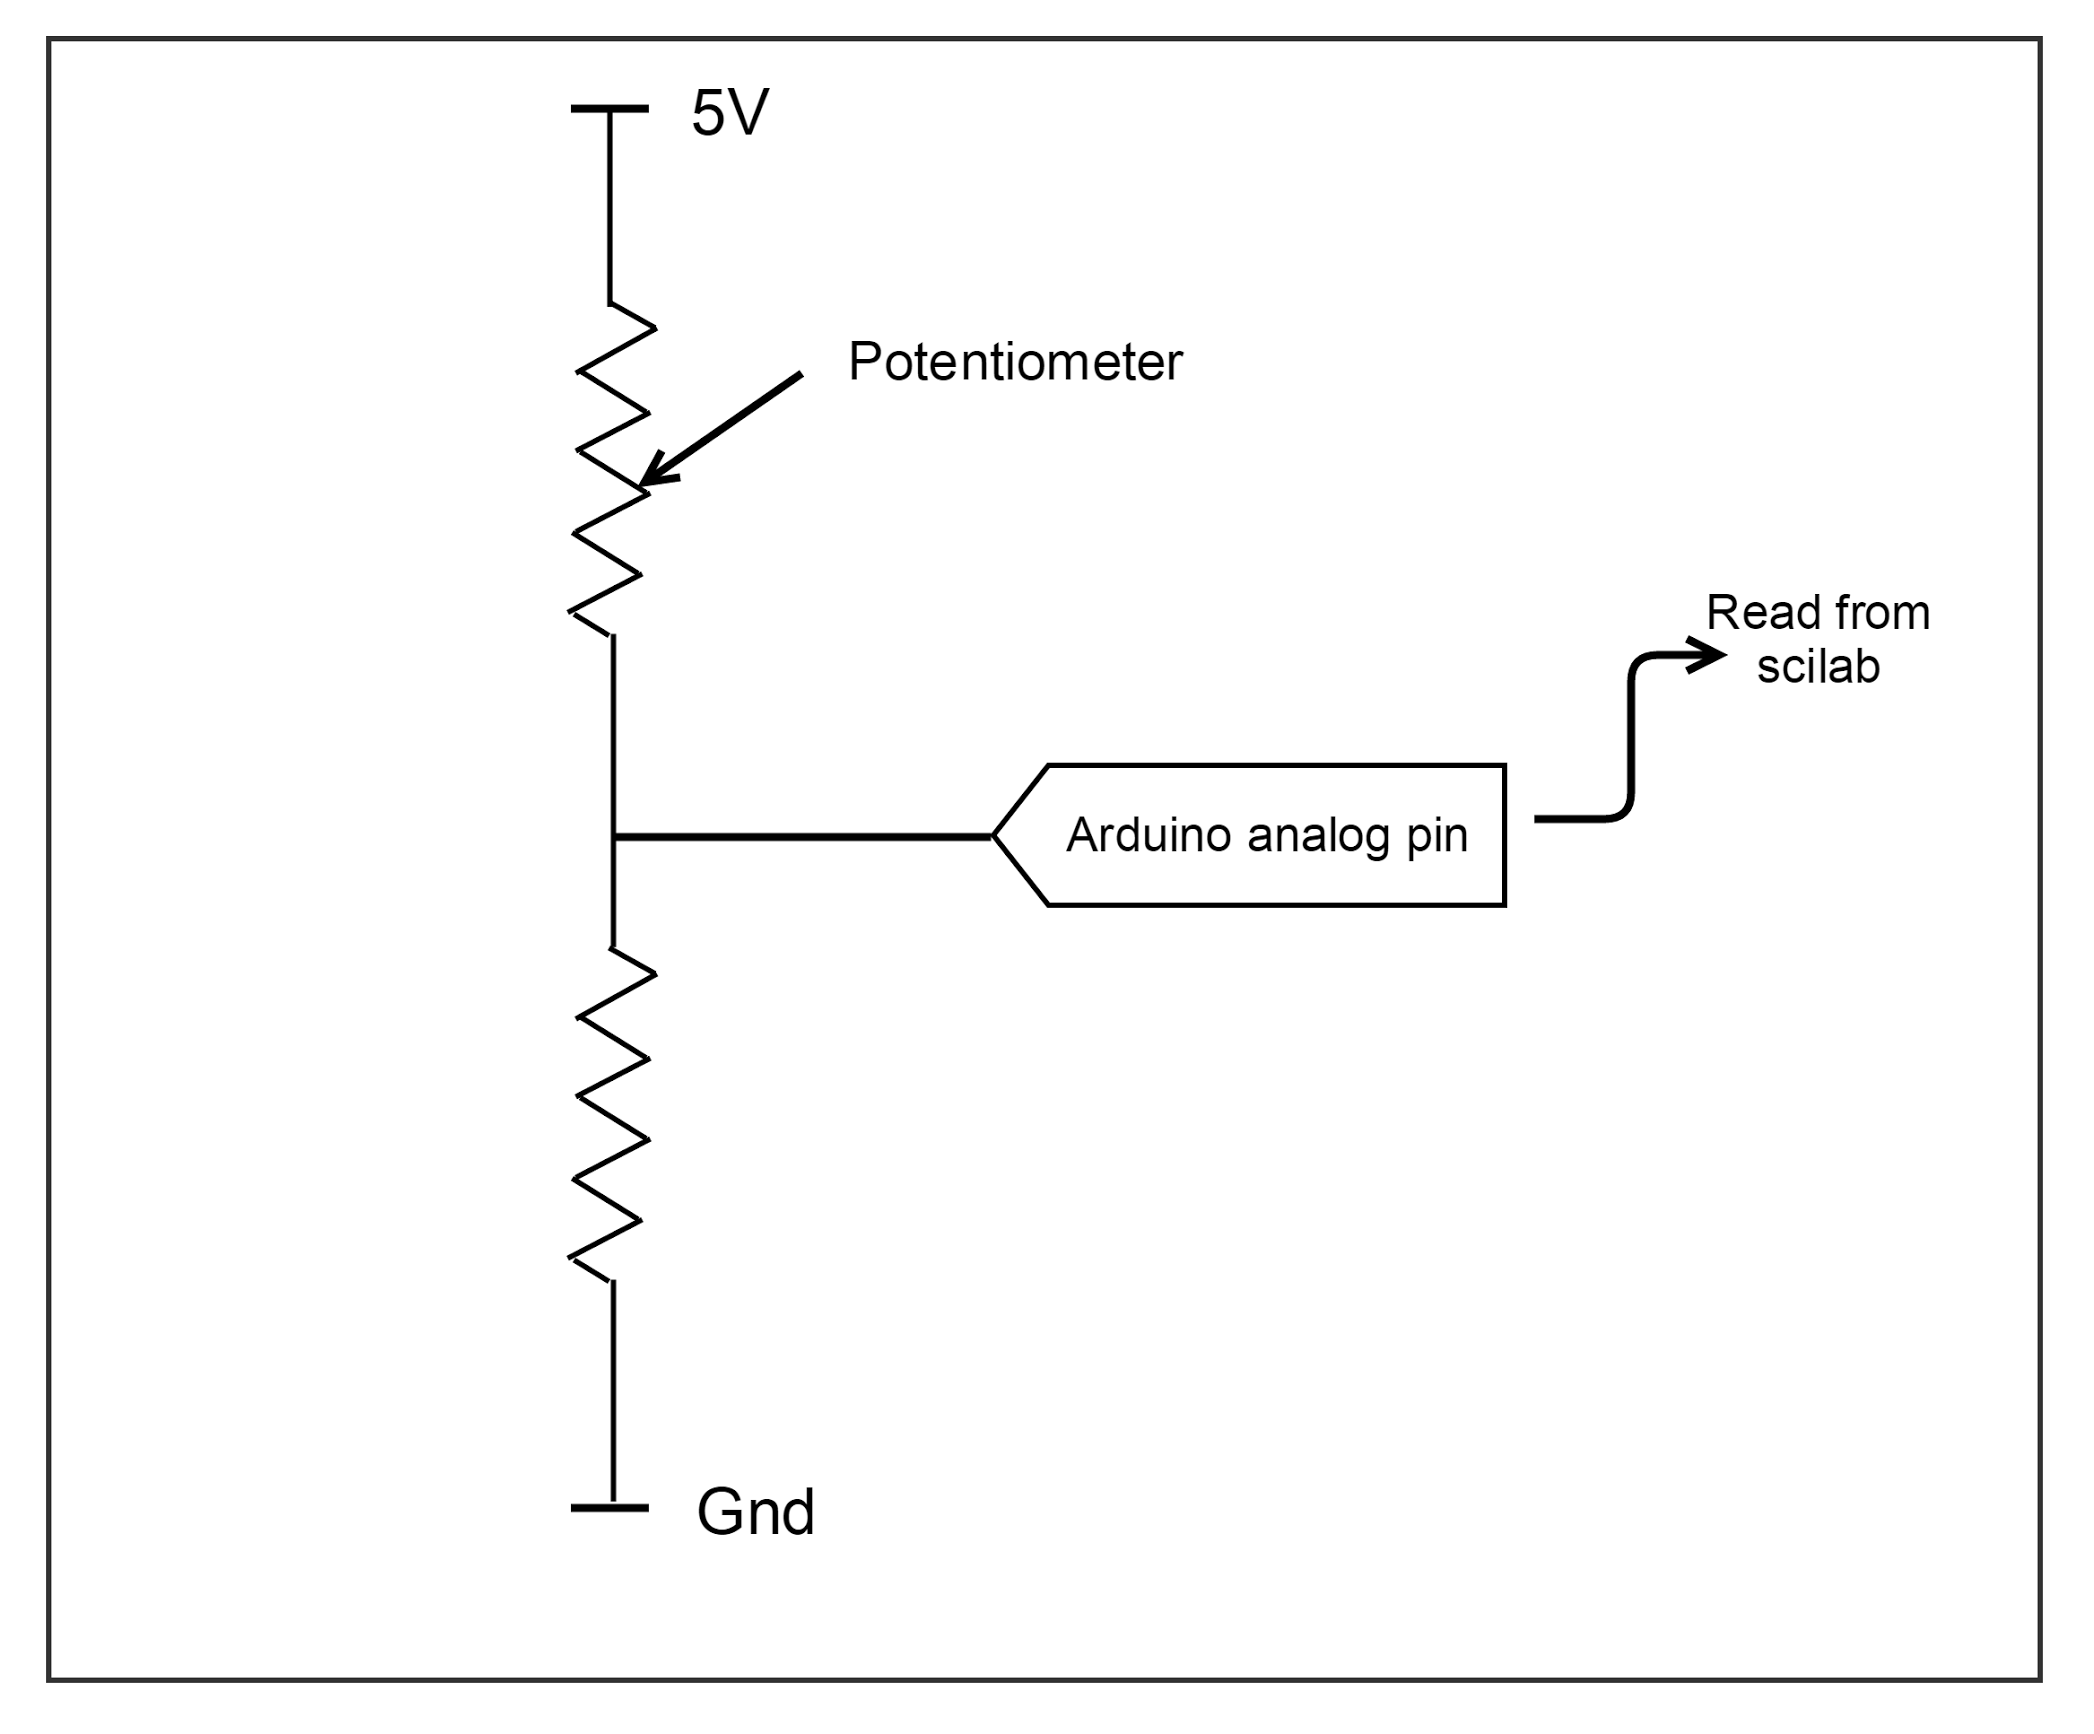
\includegraphics[width=\smfig]{\LocPotfig/potmeter.png}
\label{fig:pot}} \hfill
\subfloat[Schematic representation of the potentiometer]{
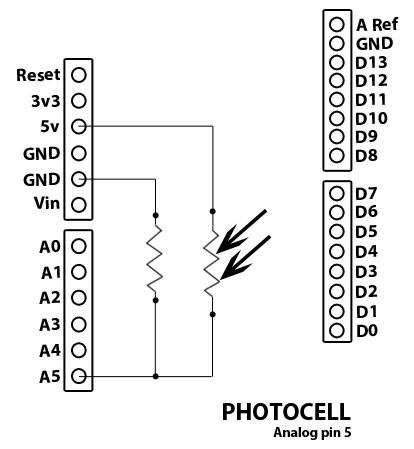
\includegraphics[width=\smfig]{\LocPotfig/schematic.png}
\label{fig:potsch}}
\caption{Potentiometer's schematic on the shield}
\label{fig:potmeterconn}
\end{figure}

The potentiometer used in the kit can be seen on the shield in
\figrefp{fig:uno-shield-connect}.  It is
mounted on the shield. The two end terminals of the potentiometer are
connected to 5V supply and ground. The middle terminal is connected to
analog pin 2 of the \arduino\ board. The resistance between the middle
terminal and either of the two ends can be varied by rotating the
middle terminal by hand. The connection diagram for the potentiometer
is shown in \figref{fig:potmeterconn}.

The reading of a potentiometer is an analog voltage varying from 0 to
5V. As for LDR, we use the ADC functionality of the
\arduino\ board. Thus, we obtain digital values between 0 and 1023 in
Scilab Console or Arduino Serial Monitor.
% redcolor{Arduino Serial Monitor}
In the experiment explained in this chapter, we shall also use an RGB
LED mounted on the shield. An RGB LED is a tri-color LED which can
illuminate in Red, GREEN and Blue colors. It has 4 leads of which one
lead is connected to ground and other three leads are connected to
digital I/O pins 9,10 and 11 of Arduino. In order to switch on a
particular LED, we need to provide HIGH(5V) voltage to the
corresponding pin of the \arduino\ board.

\section{Connecting a potentiometer with \arduino\ using a breadboard}
This section is useful for those who either don't have a shield or don't want to use the shield
for performing the experiments given in this chapter. 

To know more about a pushbutton, one should watch the Spoken Tutorials on Arduino as published on 
{\tt https://spoken-tutorial.org/}. Ideally, one should go through all the
tutorials labeled as Basic. However, we strongly recommend the readers should
watch the fifth and sixth tutorials, i.e., First Arduino Program and 
Arduino with Tricolor LED and Push button.

In case you have a potentiometer, and you want to connect it with \arduino\ on a breadboard, 
please refer to \figref{fig:pot-led}. The connections given in this figure 
can be used to control an RGB LED read the status of a pushbutton. 
\begin{figure}
  \centering
  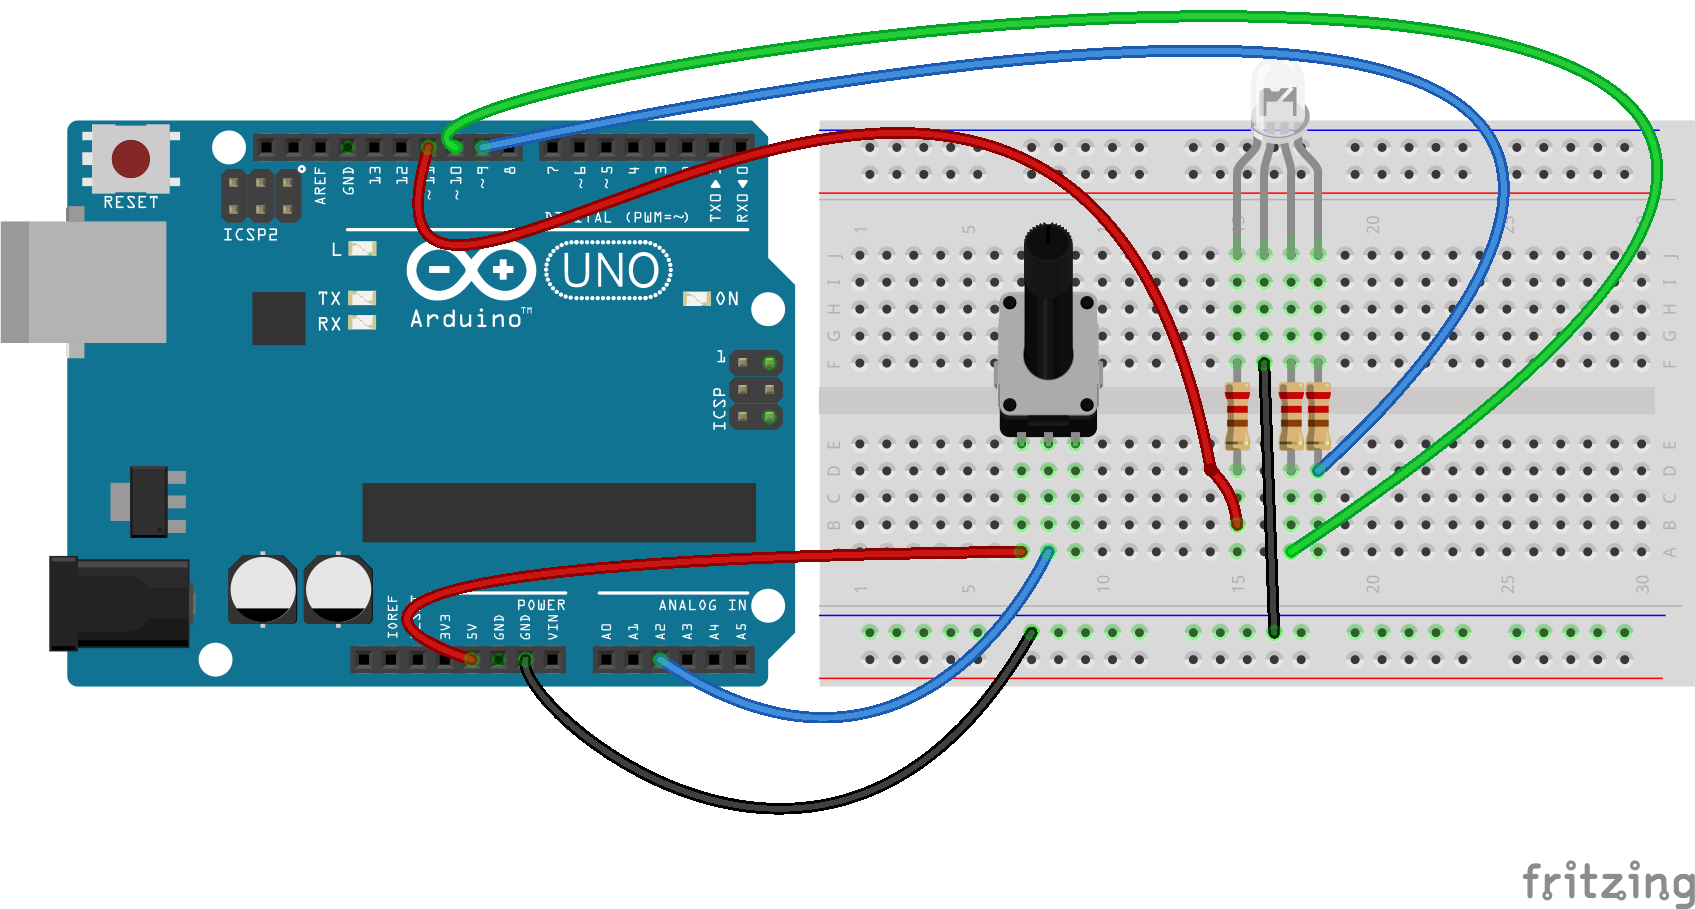
\includegraphics[width=\textwidth]{\LocPotfig/POT-led.png}
  \caption{A potentiometer to control an LED with Arduino Uno using a breadboard}
  %\redcolor{connected on pin no. D12}}
  \label{fig:pot-led}
\end{figure}
As shown in \figref{fig:pot-led}, there are three legs of the potentiometer connected to 
5V, analog pin 2, and GND on \arduino. Depending upon how much the potentiometer's shaft is rotated, one can get a value on analog pin 2. On the other hand, 
there is an RGB LED, and its four legs are connected to three different digital pins and GND on \arduino\, as discussed in 
\chapref{led}. 



\section{Reading the potentiometer from the Arduino IDE}
\subsection{Reading the potentiometer}
In this section, we shall learn to read the potentiometer input
through Arduino IDE. Depending on the acquired potentiometer values,
we will change the state of RGB LED. The Arduino code for this
experiment is given in \ardref{ard:pot-100}. Lines 1 through 4 are
used to assign relevant pin numbers to potentiometer and RGB LED. The
purpose of these lines is to avoid confusion, with the pin numbers,
for the beginners. Next, we start serial port communication, as on
line 9, with the baud rate of 115,200 bps. In order to take the
potentiometer input, we need to initialize the pins by giving the
following commands:

\lstinputlisting[firstline=10,lastline=13]
{\LocPotardcode/pot-threshold/pot-threshold.ino}

where {\tt pinMode} command is used to configure the specified pin as
an input or an output pin. The first argument for the above command
corresponds to the pin number and second argument corresponds to the
mode of operation. In this experiment, we configure digital pin 2 as
an input pin while digital pins 9, 10, and 11 as output pins. Next, we
check the value of potentiometer using {\tt analogRead} command 10
iterations. These values range from 0 to 1023. Depending on the read
value, we turn on and turn off the Red, Green or Blue LED. For
example, when the position of the potentiometer corresponds to the
values between 0 and 319, inclusive, we turn on the Red LED, keep it
on for 1000 ms and then turn it off. This functionality is carried out
by,
\lstinputlisting[firstline=18,lastline=22]
                {\LocPotardcode/pot-threshold/pot-threshold.ino}
In a similar manner,
we check the potentiometer values and correspondingly turn on and off
the Green and Blue LEDs. Note that, we used {\tt if and else if}
statements to check the conditions and rotated the potentiometer knob
to vary the resistance.

\subsection{Arduino Code}
\lstset{style=mystyle}
\label{sec:pot-arduino-code}
\addtocontents{ard}{\protect\addvspace{\codclr}}

\begin{ardcode}
  \acaption{Turning on LEDs depending on the potentiometer
    threshold}{Turning on LEDs depending on the potentiometer
    threshold.  Available at
    \LocPotardbrief{pot-threshold/pot-threshold.ino}.}
\label{ard:pot-100}
\lstinputlisting{\LocPotardcode/pot-threshold/pot-threshold.ino}
\end{ardcode}

\section{Reading the potentiometer from Scilab}
\subsection{Reading the potentiometer}
In this section, we will use a Scilab script to read the potentiometer
values.  Based on the acquired potentiometer values, we will change
the state of the RGB LED. As explained earlier, the potentiometer
values range from 0 to 1023. We will divide this entire range into 3
bands, 0-319, 320-900, and 901-1023. For each read value, we use an
{\tt if elseif} statement and correspondingly turn on either the Red,
Green or Blue LED. The code for this experiment is given in
\sciref{sci:pot-100}. We start the experiment by opening the serial
port for communication between \scilab\ and the \arduino\ board. Then,
we read the analog input at pin 2 using,
\lstinputlisting[firstline=4,lastline=4]
                {\LocPotscicode/pot-threshold.sce} where the first
                argument is for
%\redcolor {the kit number } 
the kit number and the second argument corresponds to the analog pin to be read.  Next, we compare the read values with the set range, and then turn on and off the corresponding LED. For example, 
\lstinputlisting[firstline=8,lastline=12]
{\LocPotscicode/pot-threshold.sce} where {\tt cmd\_digital\_out} is used to set the pin 11 high (1) or low (0). We used {\tt sleep(1000)} to retain the LED in the on state for 1000 milliseconds.  A similar check is done the other two bands. Note that we need to vary the resistance by rotating the knob of the potentiometer.

\subsection{Scilab Code}
\label{sec:pot-scilab-code}
\addtocontents{cod}{\protect\addvspace{\codclr}}
\begin{scicode}
  \ccaption{Turning on LEDs depending on the potentiometer
    threshold}{Turning on LEDs depending on the potentiometer
    threshold.  Available at
  \LocPotscibrief{pot-threshold.sce}.}
\label{sci:pot-100}
\lstinputlisting{\LocPotscicode/pot-threshold.sce}
\end{scicode}

\section{Reading the potentiometer from Xcos}
In this section, we discuss how to perform the experiment explained
above.  When the file required for this experiment is invoked, one
gets the GUI as in \figref{fig:pot-threshold}.  In the caption of this
figure, one can see where to locate the file.  The reader should go
through the instructions given in \secref{sec:xcos-start} before
getting started.

The block, Analog Read Pin 2, performs the read operation from pin 2. The threshold is set using the block, Dynamic. Depending on the condition met, a $1$ or $0$ is given to pin 9, 10 or 11.
\begin{figure}
  \centering
  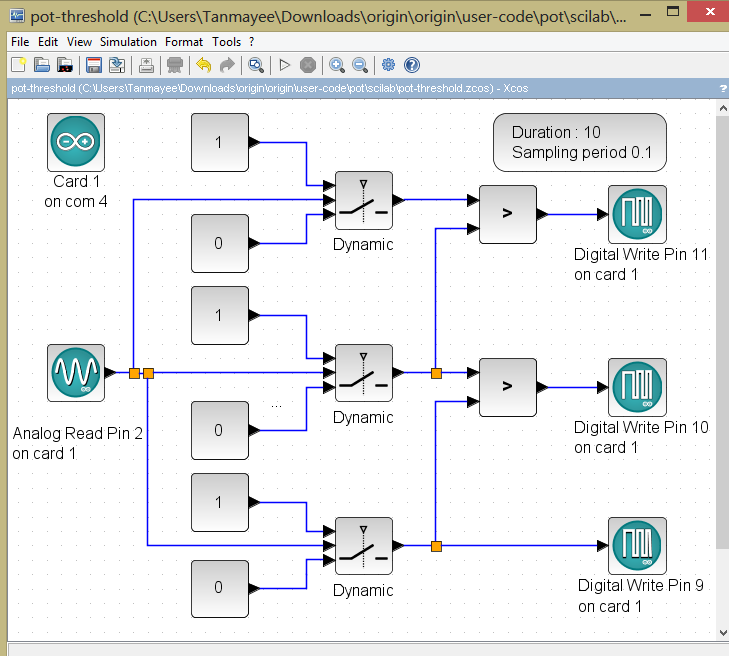
\includegraphics[width=\lgfig]{\LocPotfig/pot-threshold.PNG}
  \caption[Turning LEDs on through Xcos depending on the potentiometer
  threshold]{Turning LEDs on through Xcos depending on the
    potentiometer threshold.  This is what one sees when
      \LocPotscibrief{pot-threshold.zcos}, is invoked.}
  \label{fig:pot-threshold}
\end{figure}

We will next explain how to set the parameters for this simulation.
To set value on any block, one needs to right click and open the {\tt
  Block Parameters} or double click.  The values for each block is
tabulated in \tabref{tab:pot-threshold}.  All other parameters are to
be left unchanged.
  \begin{table}
    \centering
    \caption{Xcos parameters to turn on different LEDs depending on the
      potentiometer value}
    \label{tab:pot-threshold}
    \begin{tabular}{llc} \hline
      Name of the block & Parameter name & Value \\ \hline
      ARDUINO\_SETUP & Identifier of Arduino Card & 1 \\
      & Serial com port number & 2\portcmd \\ \hline
      TIME\_SAMPLE & Duration of acquisition(s) & 10 \\
      & Sampling period(s) & 0.1 \\ \hline
      CONST\_m & Constant Value & 1, 0 \\ \hline
      DIGITAL\_WRITE\_SB & Digital Pin & 9(blue) \\
      & Digital Pin & 10(green) \\
      & Digital Pin & 11(red) \\ 
      & Arduino card number & 1 \\ \hline
      ANALOG\_READ\_SB & analog pin & 2 \\
      & Arduino card number & 1 \\ \hline
      SWITCH2\_m & Datatype & 1 \\
      & Pass first input & 1 \\
      & threshold & 0 \\
      & use zero crossing & 1 \\ \hline
      SWITCH2\_m & Datatype & 1 \\
      & Pass first input & 0 \\
      & threshold & 320 \\
      & use zero crossing & 1 \\ \hline
      SWITCH2\_m & Datatype & 1 \\
      & Pass first input & 0 \\
      & threshold & 900 \\
      & use zero crossing & 1 \\ \hline
      RELATIONALOP & Operator & 4 \\
      & zero crossing & 0 \\
      & Datatype & 1 \\ \hline
    \end{tabular}
  \end{table}


Note that, when the potentiometer value read by Scilab crosses either
of the thresholds, color of the LED changes. This can be observed by
rotating the potentiometer.

\paragraph{Exercise:}
List out the applications in day to day life where potentiometer is
being used/can be used? For example, old fan regulators used
potentiometer to change the fan speed.

\section{Reading the potentiometer from Python}
\subsection{Reading the potentiometer}
In this section, we will use a Python script to read the potentiometer
values.  Based on the acquired potentiometer values, we will change
the state of the RGB LED. As explained earlier, the potentiometer
values range from 0 to 1023. We will divide this entire range into 3
bands, 0-319, 320-900, and 901-1023. For each read value, we use an
{\tt if elseif} statement and correspondingly turn on either the Red,
Green or Blue LED. The code for this experiment is given in
\pyref{py:pot-100}. We start the experiment by opening the serial port
for communication between python and the arduino board. Then, we read
the analog input at pin 2 using,
\lstinputlisting[firstline=4,lastline=4]
                {\LocPotpycode/pot-threshold.py} where the first
                argument is for
%\redcolor {the kit number } 
the kit number and the second argument corresponds to the analog pin to be read.  Next, we compare the read values with the set range, and then turn on and off the corresponding LED. For example, 
\lstinputlisting[firstline=8,lastline=12]
{\LocPotpycode/pot-threshold.py} where {\tt cmd\_digital\_out} is used to set the pin 11 high (1) or low (0). We used {\tt sleep(1000)} to retain the LED in the on state for 1000 milliseconds.  A similar check is done the other two bands. Note that we need to vary the resistance by rotating the knob of the potentiometer.

\subsection{Python Code}
\label{sec:pot-python-code}
\addtocontents{pyd}{\protect\addvspace{\codclr}}
\begin{pycode}
  \pcaption{Turning on LEDs depending on the potentiometer
    threshold}{Turning on LEDs depending on the potentiometer
    threshold.  Available at
  \LocPotpybrief{pot-threshold.py}.}
\label{py:pot-100}
\lstinputlisting{\LocPotpycode/pot-threshold.py}
\end{pycode}

\section{Reading the potentiometer from Julia}
\subsection{Reading the potentiometer}
In this section, we will use a Julia script to read the potentiometer values.  Based on the acquired potentiometer values, we will change the state of the RGB LED as explained earlier.The code for this experiment is given in
\juliaref{julia:pot-100}. We start the experiment by opening the serial port for communication between julia and the arduino board. Then, we read the analog input at pin 2 using,
\lstinputlisting[firstline=9,lastline=9]
{\LocPotjuliacode/pot-threshold.jl} where the first argument is for
%\redcolor {the kit number } 
the serial port and the second argument corresponds to the analog pin to be read.  Next, we compare the read values with the set range, and then turn on and off the corresponding LED. For example, 
\lstinputlisting[firstline=10,lastline=13]
{\LocPotjuliacode/pot-threshold.jl} where {\tt digiWrite} is used to set the pin 11 high (1) or low (0). We used {\tt sleep(1000)} to retain the LED in the on state for 1 second.  A similar check is done the other two bands. Note that we need to vary the resistance by rotating the knob of the potentiometer.

\subsection{Julia Code}
\label{sec:pot-julia-code}
\addtocontents{juliad}{\protect\addvspace{\codclr}}
\begin{juliacode}
  \jcaption{Turning on LEDs depending on the potentiometer
    threshold}{Turning on LEDs depending on the potentiometer
    threshold.  Available at
  \LocPotjuliabrief{pot-threshold.jl}.}
\label{julia:pot-100}
\lstinputlisting{\LocPotjuliacode/pot-threshold.jl}
\end{juliacode}

\section{Reading the potentiometer from OpenModelica}
\subsection{Reading the potentiometer}
In this section, we will use a OpenModelica script to read the potentiometer values.  Based on the acquired potentiometer values, we will change the state of the RGB LED as explained earlier.The code for this experiment is given in
\OpenModelicaref{OpenModelica:pot-100}. We start the experiment by opening the serial port for communication between OpenModelica and the arduino board. Then, we read the analog input at pin 2 using,
\lstinputlisting[firstline=17,lastline=17]
{\LocPotOpenModelicacode/pot-threshold.mo} where the first argument is for
%\redcolor {the kit number } 
the serial port and the second argument corresponds to the analog pin to be read.  Next, we compare the read values with the set range, and then turn on and off the corresponding LED. For example, 
\lstinputlisting[firstline=20,lastline=22]
{\LocPotOpenModelicacode/pot-threshold.mo} where {\tt cmd\_digital\_out} is used to set the pin 11 high (1) or low (0). We used {\tt delay(1000)} to retain the LED in the on state for 1 second.  A similar check is done the other two bands. Note that we need to vary the resistance by rotating the knob of the potentiometer.

\subsection{OpenModelica Code}
\label{sec:pot-OpenModelica-code}
\addtocontents{OpenModelicad}{\protect\addvspace{\codclr}}
\begin{OpenModelicacode}
  \mcaption{Turning on LEDs depending on the potentiometer
    threshold}{Turning on LEDs depending on the potentiometer
    threshold.  Available at
  \LocPotOpenModelicabrief{pot-threshold.mo}.}
\label{OpenModelica:pot-100}
\lstinputlisting{\LocPotOpenModelicacode/pot-threshold.mo}
\end{OpenModelicacode}
